\documentclass{standalone}
\usepackage{tikz}
\usetikzlibrary{patterns, positioning}


\begin{document}
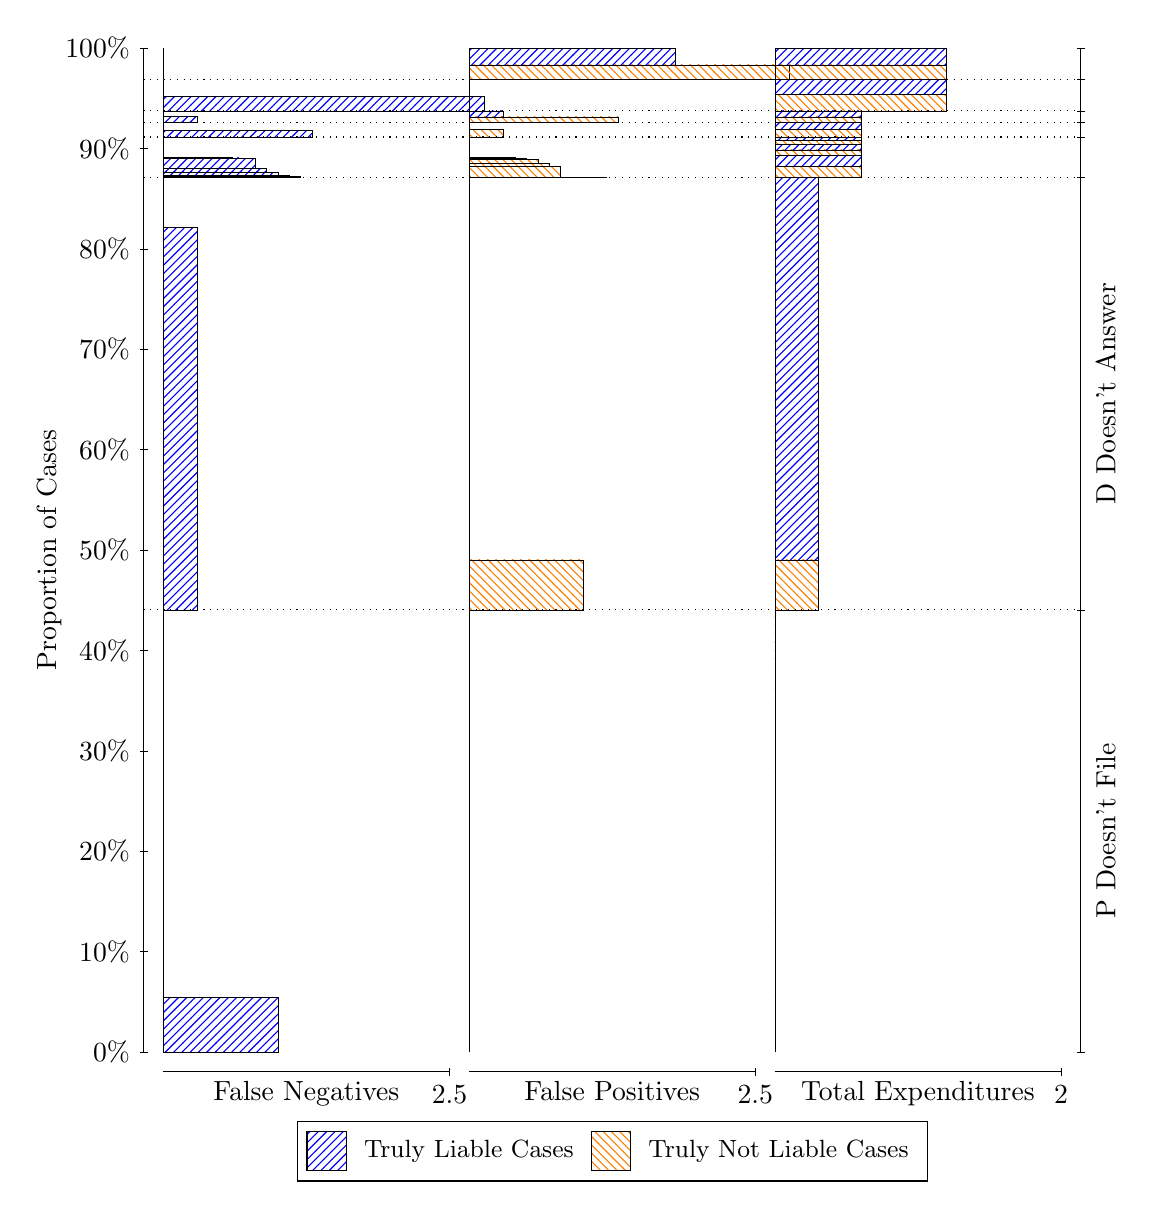
\begin{tikzpicture}
\draw[black, very thin] (1.5,1.75) -- (1.5,14.5);
\node[rotate=90, text=black, anchor=center] at (0.3, 8.125) {Proportion of Cases};
\draw[black, very thin] (1.45,1.75) -- (1.55,1.75);
\node[text=black, anchor=east] at (1.45, 1.75) {0\%};
\draw[black, very thin] (1.45,3.025) -- (1.55,3.025);
\node[text=black, anchor=east] at (1.45, 3.025) {10\%};
\draw[black, very thin] (1.45,4.3) -- (1.55,4.3);
\node[text=black, anchor=east] at (1.45, 4.3) {20\%};
\draw[black, very thin] (1.45,5.575) -- (1.55,5.575);
\node[text=black, anchor=east] at (1.45, 5.575) {30\%};
\draw[black, very thin] (1.45,6.85) -- (1.55,6.85);
\node[text=black, anchor=east] at (1.45, 6.85) {40\%};
\draw[black, very thin] (1.45,8.125) -- (1.55,8.125);
\node[text=black, anchor=east] at (1.45, 8.125) {50\%};
\draw[black, very thin] (1.45,9.4) -- (1.55,9.4);
\node[text=black, anchor=east] at (1.45, 9.4) {60\%};
\draw[black, very thin] (1.45,10.675) -- (1.55,10.675);
\node[text=black, anchor=east] at (1.45, 10.675) {70\%};
\draw[black, very thin] (1.45,11.95) -- (1.55,11.95);
\node[text=black, anchor=east] at (1.45, 11.95) {80\%};
\draw[black, very thin] (1.45,13.225) -- (1.55,13.225);
\node[text=black, anchor=east] at (1.45, 13.225) {90\%};
\draw[black, very thin] (1.45,14.5) -- (1.55,14.5);
\node[text=black, anchor=east] at (1.45, 14.5) {100\%};

\draw[black, very thin] (13.4,1.75) -- (13.4,14.5);
\draw[black, very thin] (13.35,1.75) -- (13.45,1.75);
\node[anchor=west] at (13.35, 1.75) {};
\draw[black, very thin] (13.35,7.3641) -- (13.45,7.3641);
\node[anchor=west] at (13.35, 7.3641) {};
\draw[black, very thin] (13.35,12.853) -- (13.45,12.853);
\node[anchor=west] at (13.35, 12.853) {};
\draw[black, very thin] (13.35,13.37) -- (13.45,13.37);
\node[anchor=west] at (13.35, 13.37) {};
\draw[black, very thin] (13.35,13.554) -- (13.45,13.554);
\node[anchor=west] at (13.35, 13.554) {};
\draw[black, very thin] (13.35,13.703) -- (13.45,13.703);
\node[anchor=west] at (13.35, 13.703) {};
\draw[black, very thin] (13.35,14.099) -- (13.45,14.099);
\node[anchor=west] at (13.35, 14.099) {};
\draw[black, very thin] (13.35,14.5) -- (13.45,14.5);
\node[anchor=west] at (13.35, 14.5) {};

\draw[black, very thin, pattern color=blue, pattern=north east lines] (1.75,1.75) rectangle (3.2033,2.4474);
\draw[black, very thin, pattern color=orange, pattern=north west lines] (1.75,2.4474) rectangle (1.75,7.3641);
\draw[black, very thin, pattern color=blue, pattern=north east lines] (1.75,7.3641) rectangle (2.186,12.218);
\draw[black, very thin, pattern color=orange, pattern=north west lines] (1.75,12.218) rectangle (1.75,12.853);
\draw[black, very thin, pattern color=blue, pattern=north east lines] (1.75,12.853) rectangle (3.494,12.866);
\draw[black, very thin, pattern color=blue, pattern=north east lines] (1.75,12.866) rectangle (3.3487,12.878);
\draw[black, very thin, pattern color=blue, pattern=north east lines] (1.75,12.878) rectangle (3.2033,12.925);
\draw[black, very thin, pattern color=blue, pattern=north east lines] (1.75,12.925) rectangle (3.058,12.926);
\draw[black, very thin, pattern color=blue, pattern=north east lines] (1.75,12.926) rectangle (3.058,12.967);
\draw[black, very thin, pattern color=blue, pattern=north east lines] (1.75,12.967) rectangle (2.9127,13.103);
\draw[black, very thin, pattern color=blue, pattern=north east lines] (1.75,13.103) rectangle (2.7673,13.105);
\draw[black, very thin, pattern color=blue, pattern=north east lines] (1.75,13.105) rectangle (2.622,13.108);
\draw[black, very thin, pattern color=blue, pattern=north east lines] (1.75,13.108) rectangle (2.4767,13.109);
\draw[black, very thin, pattern color=blue, pattern=north east lines] (1.75,13.109) rectangle (2.3313,13.111);
\draw[black, very thin, pattern color=orange, pattern=north west lines] (1.75,13.111) rectangle (1.75,13.37);
\draw[black, very thin, pattern color=blue, pattern=north east lines] (1.75,13.37) rectangle (3.6393,13.458);
\draw[black, very thin, pattern color=orange, pattern=north west lines] (1.75,13.458) rectangle (1.75,13.554);
\draw[black, very thin, pattern color=blue, pattern=north east lines] (1.75,13.554) rectangle (2.186,13.631);
\draw[black, very thin, pattern color=orange, pattern=north west lines] (1.75,13.631) rectangle (1.75,13.703);
\draw[black, very thin, pattern color=blue, pattern=north east lines] (1.75,13.703) rectangle (5.8193,13.89);
\draw[black, very thin, pattern color=orange, pattern=north west lines] (1.75,13.89) rectangle (1.75,14.099);
\draw[black, very thin, pattern color=orange, pattern=north west lines] (1.75,14.099) rectangle (1.75,14.286);
\draw[black, very thin, pattern color=blue, pattern=north east lines] (1.75,14.286) rectangle (1.75,14.5);
\draw[black, very thin, pattern color=orange, pattern=north west lines] (5.6333,1.75) rectangle (5.6333,6.6666);
\draw[black, very thin, pattern color=blue, pattern=north east lines] (5.6333,6.6666) rectangle (5.6333,7.3641);
\draw[black, very thin, pattern color=orange, pattern=north west lines] (5.6333,7.3641) rectangle (7.0867,7.9996);
\draw[black, very thin, pattern color=blue, pattern=north east lines] (5.6333,7.9996) rectangle (5.6333,12.853);
\draw[black, very thin, pattern color=orange, pattern=north west lines] (5.6333,12.853) rectangle (7.3773,12.855);
\draw[black, very thin, pattern color=orange, pattern=north west lines] (5.6333,12.855) rectangle (7.232,12.855);
\draw[black, very thin, pattern color=orange, pattern=north west lines] (5.6333,12.855) rectangle (7.0867,12.859);
\draw[black, very thin, pattern color=orange, pattern=north west lines] (5.6333,12.859) rectangle (6.9413,12.861);
\draw[black, very thin, pattern color=orange, pattern=north west lines] (5.6333,12.861) rectangle (6.796,12.997);
\draw[black, very thin, pattern color=orange, pattern=north west lines] (5.6333,12.997) rectangle (6.6507,13.039);
\draw[black, very thin, pattern color=orange, pattern=north west lines] (5.6333,13.039) rectangle (6.5053,13.086);
\draw[black, very thin, pattern color=orange, pattern=north west lines] (5.6333,13.086) rectangle (6.36,13.098);
\draw[black, very thin, pattern color=orange, pattern=north west lines] (5.6333,13.098) rectangle (6.2147,13.112);
\draw[black, very thin, pattern color=blue, pattern=north east lines] (5.6333,13.112) rectangle (5.924,13.114);
\draw[black, very thin, pattern color=blue, pattern=north east lines] (5.6333,13.114) rectangle (5.7787,13.115);
\draw[black, very thin, pattern color=blue, pattern=north east lines] (5.6333,13.115) rectangle (5.6333,13.37);
\draw[black, very thin, pattern color=orange, pattern=north west lines] (5.6333,13.37) rectangle (6.0693,13.465);
\draw[black, very thin, pattern color=blue, pattern=north east lines] (5.6333,13.465) rectangle (5.6333,13.554);
\draw[black, very thin, pattern color=orange, pattern=north west lines] (5.6333,13.554) rectangle (7.5227,13.625);
\draw[black, very thin, pattern color=blue, pattern=north east lines] (5.6333,13.625) rectangle (6.0693,13.703);
\draw[black, very thin, pattern color=orange, pattern=north west lines] (5.6333,13.703) rectangle (5.6333,13.912);
\draw[black, very thin, pattern color=blue, pattern=north east lines] (5.6333,13.912) rectangle (5.6333,14.099);
\draw[black, very thin, pattern color=orange, pattern=north west lines] (5.6333,14.099) rectangle (9.7027,14.286);
\draw[black, very thin, pattern color=blue, pattern=north east lines] (5.6333,14.286) rectangle (8.2493,14.5);
\draw[black, very thin, pattern color=orange, pattern=north west lines] (9.5167,1.75) rectangle (9.5167,6.6666);
\draw[black, very thin, pattern color=blue, pattern=north east lines] (9.5167,6.6666) rectangle (9.5167,7.3641);
\draw[black, very thin, pattern color=orange, pattern=north west lines] (9.5167,7.3641) rectangle (10.062,7.9996);
\draw[black, very thin, pattern color=blue, pattern=north east lines] (9.5167,7.9996) rectangle (10.062,12.853);
\draw[black, very thin, pattern color=orange, pattern=north west lines] (9.5167,12.853) rectangle (10.607,12.993);
\draw[black, very thin, pattern color=blue, pattern=north east lines] (9.5167,12.993) rectangle (10.607,13.133);
\draw[black, very thin, pattern color=orange, pattern=north west lines] (9.5167,13.133) rectangle (10.607,13.207);
\draw[black, very thin, pattern color=blue, pattern=north east lines] (9.5167,13.207) rectangle (10.607,13.279);
\draw[black, very thin, pattern color=orange, pattern=north west lines] (9.5167,13.279) rectangle (10.607,13.324);
\draw[black, very thin, pattern color=blue, pattern=north east lines] (9.5167,13.324) rectangle (10.607,13.37);
\draw[black, very thin, pattern color=orange, pattern=north west lines] (9.5167,13.37) rectangle (10.607,13.465);
\draw[black, very thin, pattern color=blue, pattern=north east lines] (9.5167,13.465) rectangle (10.607,13.554);
\draw[black, very thin, pattern color=orange, pattern=north west lines] (9.5167,13.554) rectangle (10.607,13.625);
\draw[black, very thin, pattern color=blue, pattern=north east lines] (9.5167,13.625) rectangle (10.607,13.703);
\draw[black, very thin, pattern color=orange, pattern=north west lines] (9.5167,13.703) rectangle (11.697,13.912);
\draw[black, very thin, pattern color=blue, pattern=north east lines] (9.5167,13.912) rectangle (11.697,14.099);
\draw[black, very thin, pattern color=orange, pattern=north west lines] (9.5167,14.099) rectangle (11.697,14.286);
\draw[black, very thin, pattern color=blue, pattern=north east lines] (9.5167,14.286) rectangle (11.697,14.5);
\draw[black, dotted] (1.5,7.3641) -- (13.4,7.3641);
\draw[black, dotted] (1.5,12.853) -- (13.4,12.853);
\draw[black, dotted] (1.5,13.37) -- (13.4,13.37);
\draw[black, dotted] (1.5,13.554) -- (13.4,13.554);
\draw[black, dotted] (1.5,13.703) -- (13.4,13.703);
\draw[black, dotted] (1.5,14.099) -- (13.4,14.099);
\draw[black, very thin] (1.75,1.5) -- (5.3833,1.5);
\node[text=black, anchor=north] at (3.5667, 1.5) {False Negatives};
\draw[black, very thin] (5.3833,1.45) -- (5.3833,1.55);
\node[text=black, anchor=north] at (5.3833, 1.45) {2.5};

\draw[black, very thin] (5.6333,1.5) -- (9.2667,1.5);
\node[text=black, anchor=north] at (7.45, 1.5) {False Positives};
\draw[black, very thin] (9.2667,1.45) -- (9.2667,1.55);
\node[text=black, anchor=north] at (9.2667, 1.45) {2.5};

\draw[black, very thin] (9.5167,1.5) -- (13.15,1.5);
\node[text=black, anchor=north] at (11.333, 1.5) {Total Expenditures};
\draw[black, very thin] (13.15,1.45) -- (13.15,1.55);
\node[text=black, anchor=north] at (13.15, 1.45) {2};

\node[text=black, centered, rotate=90] at (13.72, 4.557) {P Doesn't File};
\node[text=black, centered, rotate=90] at (13.72, 10.109) {D Doesn't Answer};






\draw (7.449999999999999,1.5) node[draw=none] (baseCoordinate) {};
\begin{scope}[align=center]
        \matrix[scale=0.5, draw=black, below=0.5cm of baseCoordinate, nodes={draw}, column sep=0.1cm]{
            \node[rectangle, draw, minimum width=0.5cm, minimum height=0.5cm, pattern color=blue, pattern=north east lines] {}; &
            \node[draw=none, font=\small, text=black] (B) {Truly Liable Cases}; &
            \node[rectangle, draw, minimum width=0.5cm, minimum height=0.5cm, pattern color=orange, pattern=north west lines] {}; &
            \node[draw=none, font=\small, text=black] (B) {Truly Not Liable Cases}; \\
            };
\end{scope}

\end{tikzpicture}
\end{document}